\documentclass[11pt,a4paper]{article}

\usepackage[left=2cm,text={17cm,24cm},top=3cm]{geometry}
\usepackage[czech]{babel}
\usepackage[utf8]{inputenc}
\usepackage[T1]{fontenc}

\usepackage{url}
\usepackage{float}
\usepackage{comment}
\usepackage{etoolbox}
\usepackage{graphicx}
\usepackage{hyperref}
\usepackage{tocloft}
\usepackage{pdfpages} % include pdf

\def\UrlBreaks{\do\/\do-\do\&\do=\do\_\do?} % URL breaking characters

\newcommand{\red}[1]{\textcolor{red}{#1}} % \red{text in red}
\newcommand{\blue}[1]{\textcolor{blue}{#1}} % \blue{text in blue}
\newcommand{\TODO}{\textbf{\textcolor{red}{TODO}}} % red bold TODO
\newcommand{\tilda}{\raisebox{0.5ex}{\texttildelow}} % command \tilda for '~' character

\graphicspath{{img/}} % path to images
\patchcmd{\thebibliography}{\section*{\refname}}{}{}{} % do not create section for bibliography
\hypersetup{
    linktoc    = all,
    colorlinks = true,
    citecolor  = green,
    linkcolor  = red,
    urlcolor   = blue,
}

\begin{document}
\nocite{*}

\begin{titlepage}

    \begin{center}
        % FIX: lines must end with '%', if not then it will result in an incorrect centering
        \vfill {%
            \Huge{%
                \textsc{%
                    Fakulta informačních technologií\\[3mm]%
                    Vysoké učení technické v~Brně%
                }%
            }%
        }%

        \hfill\\[15mm]

        \begin{figure}[!h]
            \centering
            
\includegraphics[scale=0.3]{vutbr-fit-logo.eps}
        \end{figure}

        \hfill\\[10mm]

        \Huge{
            \textbf{
                MSP
            }
        }

        \hfill\\[-10mm]

        \huge{
            \textbf{
                Statistika a pravděpodobnost
            }
        }

        \hfill\\[10mm]

        \LARGE{
            \textbf{
                Semestrální projekt
            }
        }
        \vfill

    \end{center}

        \Large{
            \noindent Zpracoval: Attila Lakatos (xlakat01)\hfill \\
             Čísla zadání: 6, 15 \\
             Cvičení - skupina: čtvrtek, 09:00 \\
             Datum: \today
        }

\end{titlepage}


\newpage

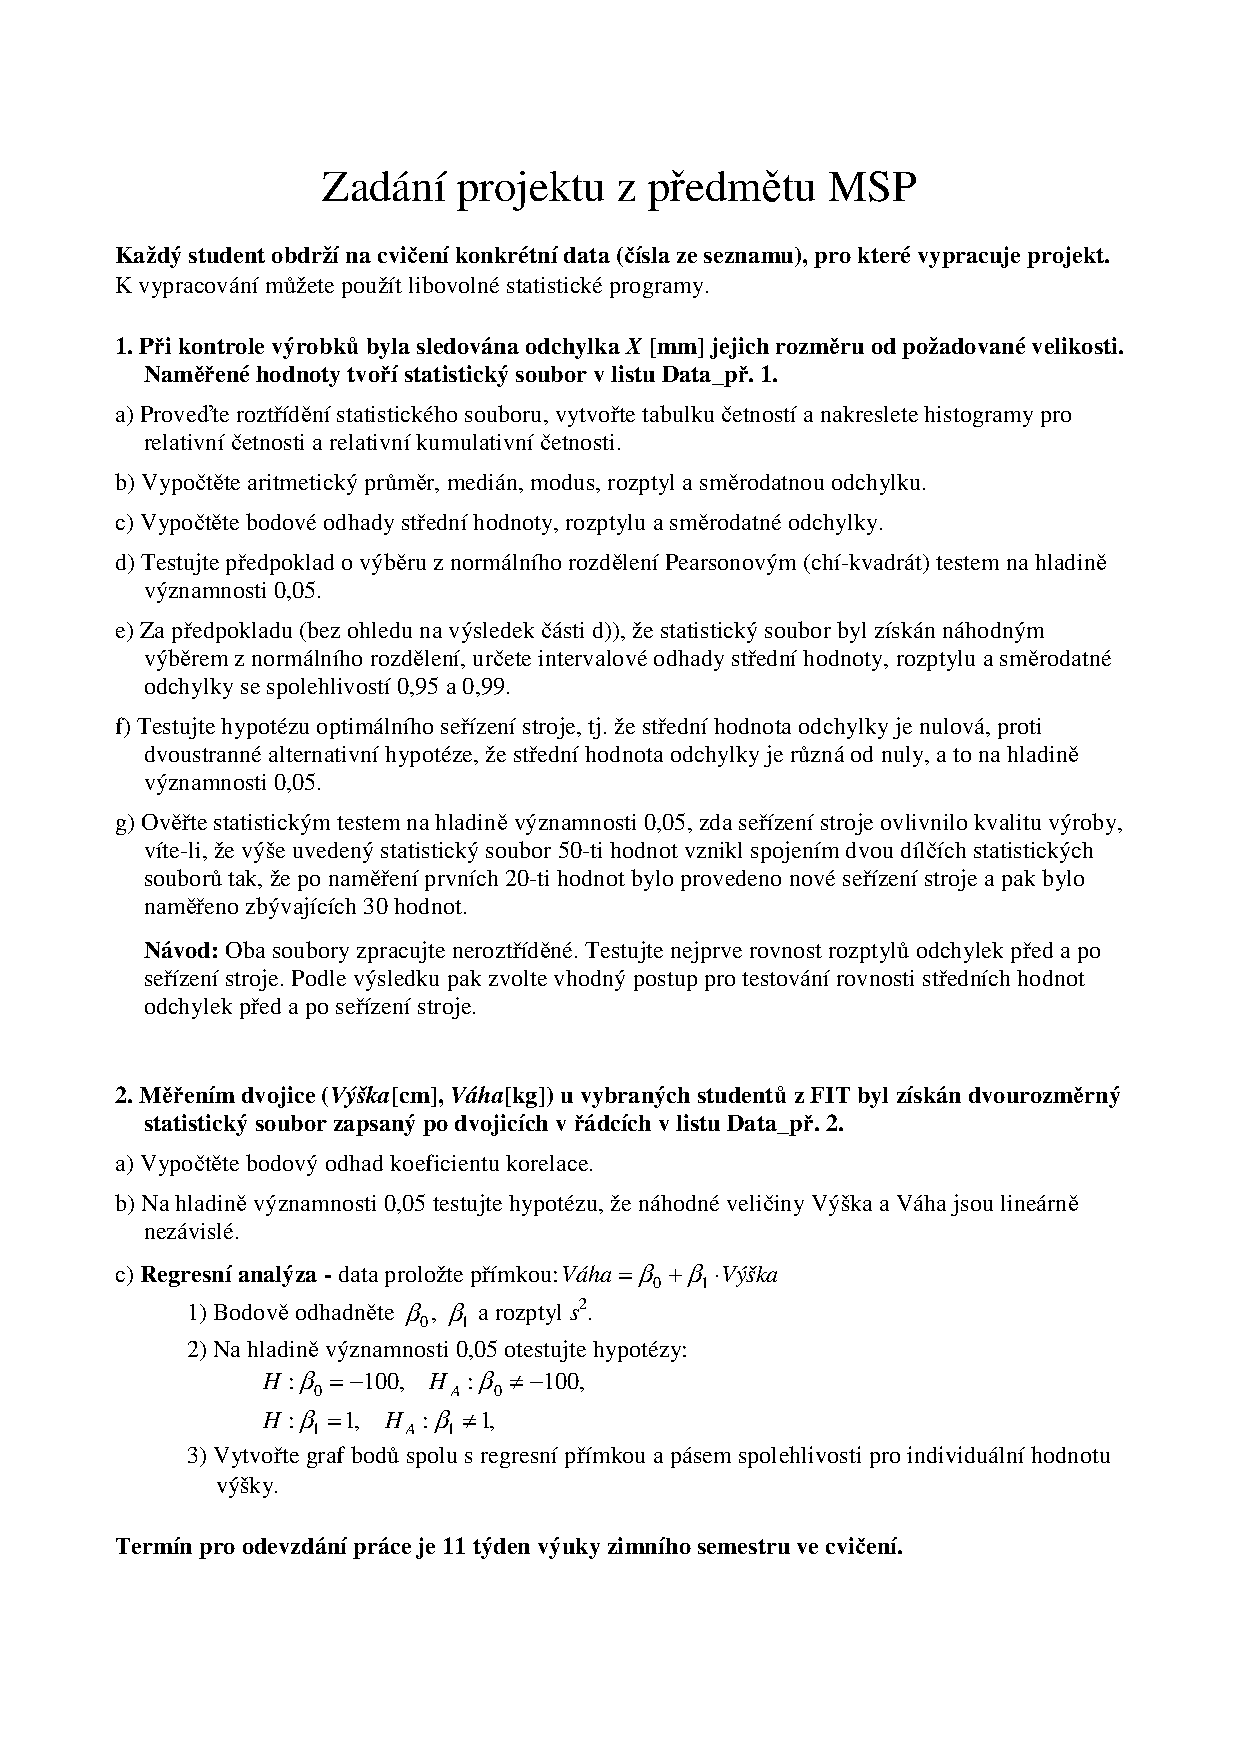
\includepdf[width=\textwidth]{img/task.pdf}

\section{Vypracování}

1. Při kontrole výrobků byla sledována odchylka X [mm] jejich rozměru od požadované velikosti. Naměřené hodnoty tvoří statistický soubor v listu Data\_př. 1.

\vspace{0,5cm}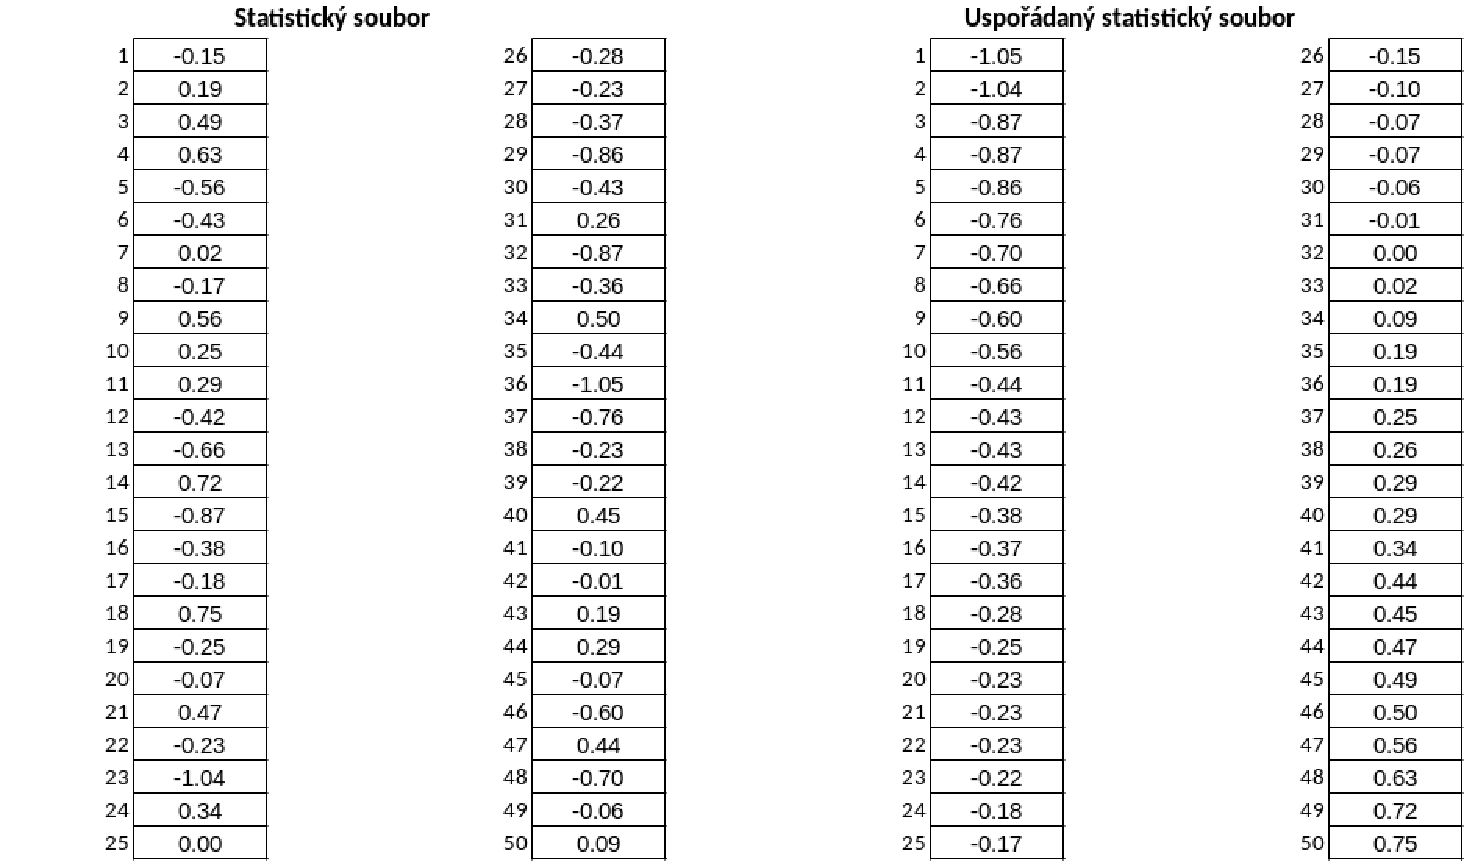
\includegraphics[width=\textwidth]{img/task1.pdf}\vspace{0,5cm}
\noindent\makebox[\linewidth]{\rule{\textwidth}{0.4pt}}
% TASK 1a

a) Proveďte roztřídění statistického souboru, vytvořte tabulku četností a nakreslete histogramy pro relativní četnosti a relativní kumulativní četnosti.
\vspace{0,5cm}

$x_{(1)} = \min\limits_i x_i = -1.05$ \\

$x_{(n)} = \max\limits_i x_i = 0.75$ \\

Variační obor: $ \langle x_{(1)}, x_{(n)} \rangle = \langle -1,05; 0,75 \rangle$ \\

Rozpětí: $ x_{(n)} - x_{(1)} = 1.8 $ \\

Počet tříd: $m = 11$ (zvoleno) \\ 

Délka třídy: $\frac{x_{(n)} - x_{(1)}}{m} = 0.163636 $

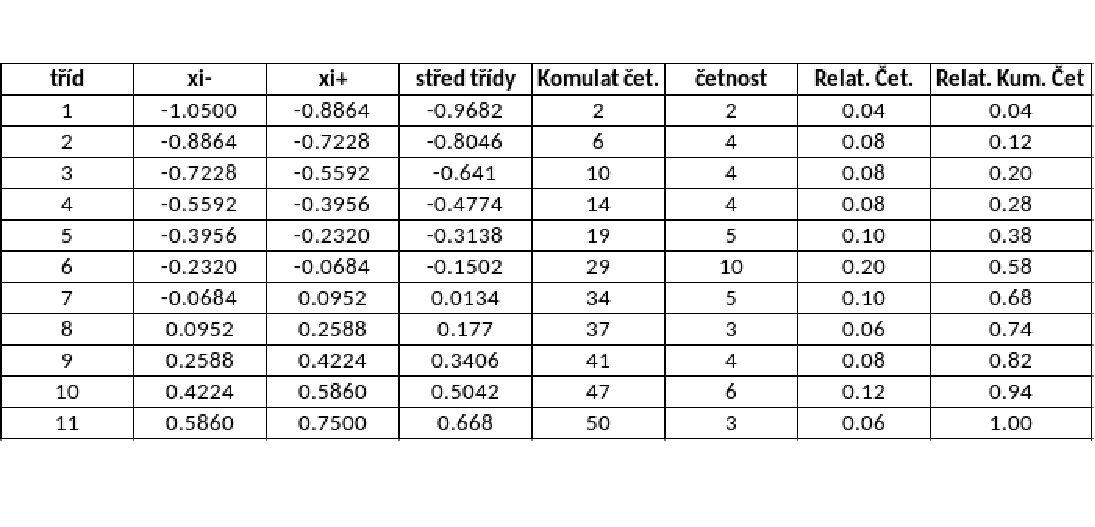
\includegraphics[width=\textwidth]{img/1atable.pdf}\vspace{-1,75cm}

\begin{figure}[H]
    \centering
    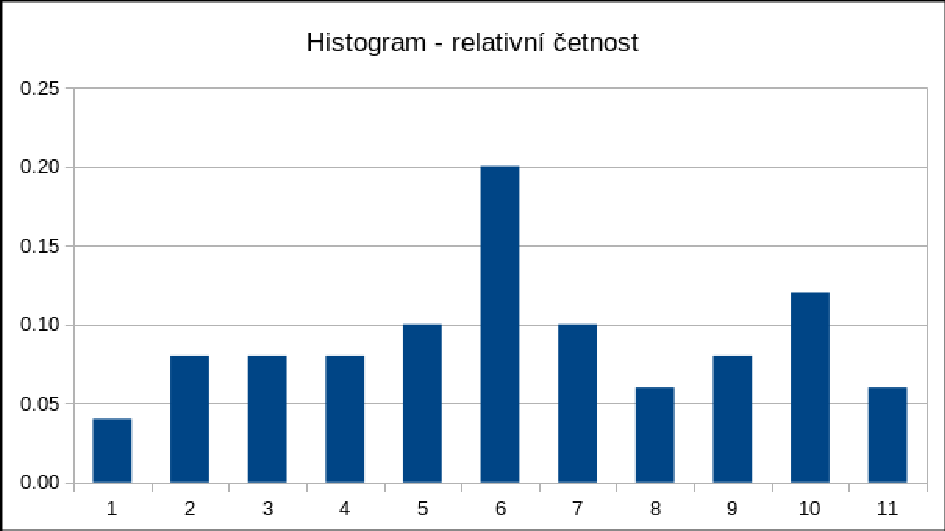
\includegraphics[width=0.55\textwidth]{img/1ahistogram1.pdf}
    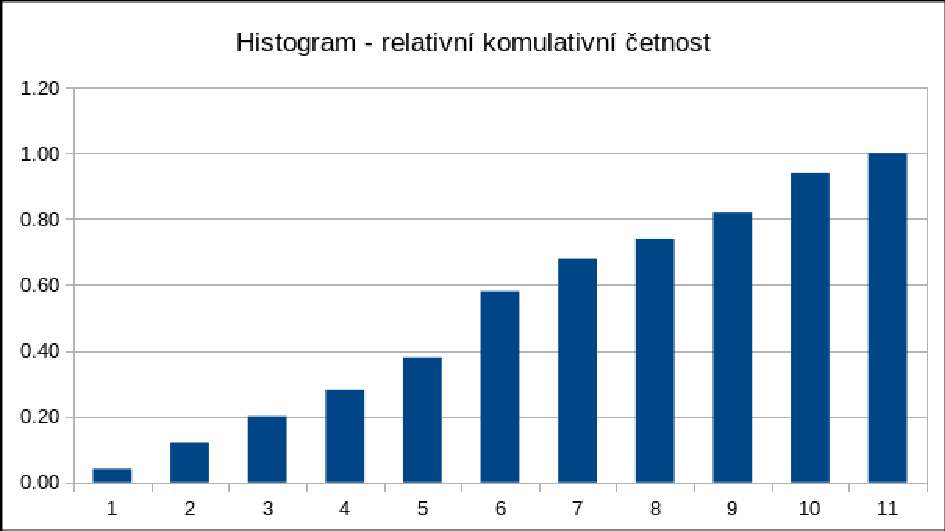
\includegraphics[width=0.55\textwidth]{img/1ahistogram2.pdf}
\end{figure}


\noindent\makebox[\linewidth]{\rule{\textwidth}{0.4pt}}
% TASK 1b

b) Vypočtěte aritmetický průměr, medián, modus, rozptyl a směrodatnou odchylku. \\

$ \overline{x} = \frac{1}{n} \sum\limits_{i=1}^n x_i = -0,1224$ \\

medián: $  \widetilde{x} = \frac{1}{2}*(-0.17 + -0.15) = 0,16 $ \\

modus: $ \widehat{x} = -0.23 (TODO) $ \\

$ s^2 = \frac{1}{n} \sum\limits_{i=1}^{n} (x_i - \overline{x})^2 = 0.21728624 $ \\

$ s = \sqrt{\frac{1}{n} \sum\limits_{i=1}^n (x_i - \overline{x})^2} = 0.466139721542801$ \\


\noindent\makebox[\linewidth]{\rule{\textwidth}{0.4pt}}
% TASK 1c

c) Vypočtěte bodové odhady střední hodnoty, rozptylu a směrodatné odchylky. \\

Bodový odhad střední hodnoty: $ \overline{x} = \frac{1}{n} \sum\limits_{i=1}^{n} x_i = -0,1224 $ \\

Bodový odhad rozptylu: $ s^2 = \frac{1}{n - 1} \sum\limits_{i=1}^{n} (x_i - \overline{x})^2 = 0.22172065306122 $ \\

Bodový odhad směrodatné odchylky: $ s = \sqrt{ \frac{1}{n - 1} \sum\limits_{i=1}^{n} (x_i - \overline{x})^2 } = 0.470872225833319 $ \\


\noindent\makebox[\linewidth]{\rule{\textwidth}{0.4pt}}
% TASK 1d

Testujte předpoklad o výběru z normálního rozdělení Pearsonovým (chí-kvadrát) testem na hladině významnosti 0,05. \\

\vspace{0.6cm}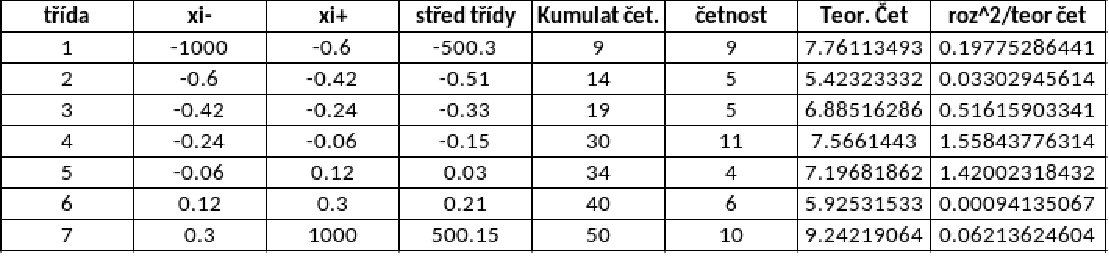
\includegraphics[width=\textwidth]{img/1dtable.pdf} \\

Testovací kritérium: $ t = \sum\limits_{j=1}^{m} \frac{(f_j - \widehat{f_j})^2}{\widehat{f_j}} = 3.788479898122$, \\

$\chi_{1-\alpha}^2$ pro $ k = 7 - 2 - 1$ stupňů volnosti: 9,488, \\

doplněk kritického oboru: $ \overline{W_{\alpha}} = \langle 0, \chi_{1-\alpha}^2 \rangle = \langle 0, 9,488 \rangle$. \\

Protože $ t \in \overline{W_{\alpha}} $, tedy hypotéza: $ X \sim N(-0,1224; 0,22172065306) $ \textbf{se nezamítá} . \\









\newpage

\section{Literatura}
\bibliographystyle{czechiso}
\begin{flushleft}
    \bibliography{quotation}
\end{flushleft}

\end{document}
